\chapter{电流强度与电流表}\label{ch:g8:intensity-ammeter}

“强电流，弱电流”——我们多年来一直这样说，
全凭感觉调节亮度与握力。今天起，感觉退休了。
电流的强弱有了名称、\omterm{def:g6:measurement-in-science:measuring}{单位}和\omterm{def:g6:measurement-in-science:measuring}{测量}仪器；
而这台仪器证明的第一条规律，
你早已隐约怀疑，却从未亲手测过。

\section{电流强度及其单位}

\begin{definition}[电流强度]\label{def:g8:intensity-ammeter:intensity}
\emph{电流强度}\index{电流强度} $I$ 衡量电流的强弱，
即每秒有多少电荷穿过电路中的某一点，
也就是电流的“流量”，正如河流的流量是每秒流过的水量。
其\omterm{def:g6:measurement-in-science:measuring}{单位}是
\emph{安培}\index{安培}（\unit{A}），以纪念一位电学先驱；
日常电路中常用
\emph{毫安}作\omterm{def:g6:measurement-in-science:measuring}{单位}：$\qty{1}{mA} = \qty{0.001}{A}$，
即千分之一安。
\end{definition}

\begin{example}[常见电流的大小]\label{ex:g8:intensity-ammeter:values}
一只小指示灯耗电约 \qty{0.02}{A} ——
即 \qty{20}{mA}；手电筒\omterm{def:g3:first-electric-circuit:bulb}{灯泡}约 \qty{0.3}{A}；汽车前大灯为
\qty{5}{A}；满功率运转的电热水壶为
\qty{10}{A}；汽车启动时，发动机从蓄\omterm{def:g3:first-electric-circuit:battery}{电池}中吸取 \qty{100}{A}；
一次闪电击中，历时仅一毫秒，却有数万
\omterm{def:g8:intensity-ammeter:intensity}{安培}的电流沿其通道猛冲而下。危险的尺度
同样发人深省：几百分之一\omterm{def:g8:intensity-ammeter:intensity}{安培}的电流穿过人体，
就足以致命——对电流的敬畏，
远在一\omterm{def:g8:intensity-ammeter:intensity}{安培}之前就该开始。
\end{example}

\begin{remark}[人名与单位]\label{rem:g8:intensity-ammeter:person}
写出来时，\omterm{def:g6:measurement-in-science:measuring}{单位}名称用小写，如“两\omterm{def:g8:intensity-ammeter:intensity}{安培}的电流”，
而大写的则是那位科学家的名字，
与所有以科学家命名的\omterm{def:g6:measurement-in-science:measuring}{单位}一样；符号 \unit{A} 保持大写。
这一约定很快还会再遇到两次。
\end{remark}

\section{电流表}

\begin{definition}[电流表]\label{def:g8:intensity-ammeter:ammeter}
\emph{电流表}\index{电流表}用来\omterm{def:g6:measurement-in-science:measuring}{测量}\omterm{def:g8:intensity-ammeter:intensity}{电流强度}，它计量
流经\emph{自身}的电流，因此必须
\emph{\omterm{def:g4:series-circuits:series}{串联}}接入所\omterm{def:g6:measurement-in-science:measuring}{测量}的回路之中，如同
公路上的收费站。为尽量少扰动电流，
它几乎不阻碍电流——这也
正是电流表若被错误地直接跨接在\omterm{def:g3:first-electric-circuit:battery}{电池}两端，
就成了一个带表盘的\omterm{def:g7:short-circuits-safety:device}{短路}：这是烧坏电流表的经典做法。
\end{definition}

\begin{method}[测量电流强度]\label{met:g8:intensity-ammeter:measure}
\begin{enumerate}
  \item 关闭电路\omterm{ex:g3:first-electric-circuit:switch}{开关}，在待测电流所在处
        \emph{断开}回路；
  \item 将\omterm{def:g8:intensity-ammeter:ammeter}{电流表}接入缺口：电流由其
        \unit{A} \omterm{def:g3:first-electric-circuit:battery}{接线柱}流入，由\emph{公共}\omterm{def:g3:first-electric-circuit:battery}{接线柱}流出，
        使电流的规定方向从电表的
        “正门”进入；
  \item 若为多量程电表，先选用\emph{最大}量程，
        再逐级调小，直至读数舒适地落在表盘上，
        以保护电表免受
        意外损坏；
  \item 闭合\omterm{ex:g3:first-electric-circuit:switch}{开关}，读数，并写上\omterm{def:g6:measurement-in-science:measuring}{单位}。
\end{enumerate}
若指针式电表接反，指针会猛撞在限位上；
数字式电表则只显示一个负号，
天天宽容着学生的粗心。
\end{method}

\begin{omfigure}
\begin{tikzpicture}[scale=0.9]
  \draw (0,0) to[battery1, l=电池] (0,2.8)
    to[short] (1.8,2.8)
    to[ammeter, l=$I$] (4.2,2.8)
    to[lamp, l=灯] (6.6,2.8)
    to[short] (8.0,2.8)
    to[short] (8.0,0)
    to[short] (0,0);
  \draw[-Stealth, very thick, omThm] (1.0,3.15) -- (1.7,3.15);
\end{tikzpicture}

{\small \omterm{def:g8:intensity-ammeter:ammeter}{电流表}在回路中占据自己的位置：如同\omterm{def:g4:series-circuits:series}{串联}在回路中的收费站，
计量着点亮\omterm{def:g3:first-electric-circuit:bulb}{灯泡}的那股电流。}
\end{omfigure}

\begin{omfigure}
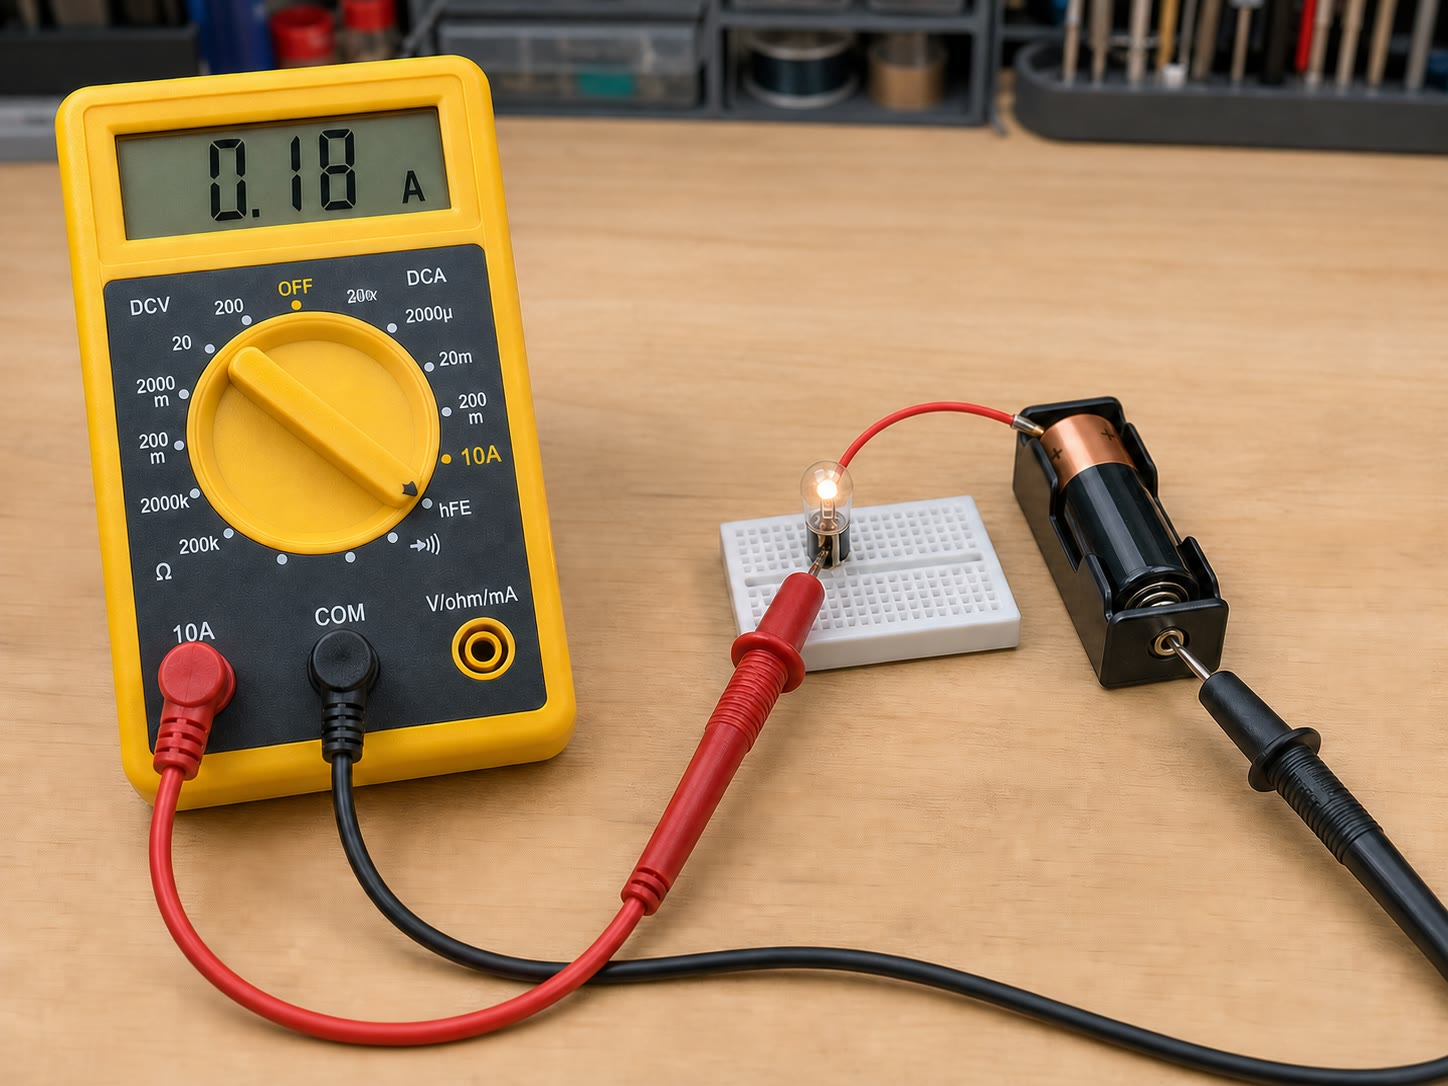
\includegraphics[width=0.5\linewidth]{images/book1/ai/g8-ammeter-multimeter.jpg}

{\small 实验台上的实物：一台仪器、两根表笔，电路中的电流便在显示屏上变为一个数字。}
\end{omfigure}

\section{第一条被测定的规律}

\begin{proposition}[同一回路，同一强度]\label{prop:g8:intensity-ammeter:sameI}
在\omterm{def:g4:series-circuits:series}{串联电路}中，回路上各点的\omterm{def:g8:intensity-ammeter:intensity}{电流强度}都相同。
将\omterm{def:g8:intensity-ammeter:ammeter}{电流表}移至任意位置——\omterm{def:g3:first-electric-circuit:bulb}{灯泡}之前、之后，
或紧靠\omterm{def:g3:first-electric-circuit:battery}{电池}，读数都不会改变。
五年来亮度相同的\omterm{def:g3:first-electric-circuit:bulb}{灯泡}所暗示的结论，
如今电表以数值予以确认：途中并无电流被消耗；
一条路，一股电流，一个 $I$。
\end{proposition}

\begin{omfigure}
\begin{tikzpicture}[scale=0.85]
  \draw (0,0) to[battery1] (0,3.0)
    to[ammeter, l=\qty{0.30}{A}] (2.6,3.0)
    to[lamp] (4.8,3.0)
    to[ammeter, l=\qty{0.30}{A}] (7.4,3.0)
    to[lamp] (9.6,3.0)
    to[short] (9.6,0)
    to[ammeter, l=\qty{0.30}{A}] (4.8,0)
    to[short] (0,0);
\end{tikzpicture}

{\small 同一回路上的三个收费站：\omterm{def:g3:first-electric-circuit:bulb}{灯泡}之前、\omterm{def:g3:first-electric-circuit:bulb}{灯泡}之间和\omterm{def:g3:first-electric-circuit:bulb}{灯泡}之后，
每个\omterm{def:g8:intensity-ammeter:ammeter}{电流表}都显示同样的 \qty{0.30}{A}。}
\end{omfigure}

\begin{example}[读懂定律的细则]\label{ex:g8:intensity-ammeter:fineprint}
定律说的是\emph{沿同一回路}，而不是\emph{对回路做的任何改动}。
若再\omterm{def:g4:series-circuits:series}{串联}一只\omterm{def:g3:first-electric-circuit:bulb}{灯泡}，电流整体减弱，
比如从 \qty{0.30}{A} 降到
\qty{0.17}{A}，但处处都\emph{同等}地减弱；
三个收费站在新数值上也一致。
同一回路，同一\omterm{def:g8:intensity-ammeter:intensity}{电流强度}——无论它此刻是多少。
\end{example}

\begin{example}[一瞥节点]\label{ex:g8:intensity-ammeter:junction}
改为在一对\omterm{def:g5:series-parallel-circuits:parallel}{并联}\omterm{def:g5:series-parallel-circuits:parallel}{支路}上设置收费站：干路
\qty{0.50}{A}；\omterm{def:g5:series-parallel-circuits:parallel}{支路}一 \qty{0.30}{A}；\omterm{def:g5:series-parallel-circuits:parallel}{支路}二
\qty{0.20}{A}。这个颇具启发性的和并非偶然——电流
流入和流出\omterm{def:g5:series-parallel-circuits:parallel}{节点}的电流必须平衡，因为电荷
在分叉路口既不会凭空产生，也不会凭空消失。完整的定律
连同与之对应的电压定律，
将在隔一章的内容中详述；你的电表其实早已接触过它。
\end{example}

\begin{remark}[万用表]\label{rem:g8:intensity-ammeter:multimeter}
车间里那块黄色的“砖头”——\emph{万用表}——把
\omterm{def:g8:intensity-ammeter:ammeter}{电流表}和其他几种仪器合并到一个机身里，靠
一个选择旋钮切换。旋钮拨到 \unit{A} 或 \unit{mA} 档，表笔插入
标有记号的插孔，它就是你的\omterm{def:g8:intensity-ammeter:ammeter}{电流表}，\omterm{def:g4:series-circuits:series}{串联}规则照样适用。
本书已有两章内容藏在其中；下一章还将引入第三类
，注意它的接线规则与之\emph{相反}。
\end{remark}

\section{练习}

\begin{exercise}[$\star$]\label{exo:g8:intensity-ammeter:1}
用“河流”的比喻来说，\omterm{def:g8:intensity-ammeter:intensity}{电流强度}\omterm{def:g6:measurement-in-science:measuring}{测量}的是什么？写出它的\omterm{def:g6:measurement-in-science:measuring}{单位}
和符号，并将 \qty{250}{mA} 换算为\omterm{def:g8:intensity-ammeter:intensity}{安培}。
\end{exercise}

\begin{exercise}[$\star$]\label{exo:g8:intensity-ammeter:2}
将\omterm{def:g8:intensity-ammeter:intensity}{电流强度}与对应场景配对：\qty{0.02}{A}；\
\qty{0.3}{A}；\ \qty{10}{A}；\ \qty{100}{A}——
分别对应电热水壶、指示灯、启动发动机、手电筒\omterm{def:g3:first-electric-circuit:bulb}{灯泡}。
\end{exercise}

\begin{exercise}[$\star$]\label{exo:g8:intensity-ammeter:3}
为什么\omterm{def:g8:intensity-ammeter:ammeter}{电流表}必须\omterm{def:g4:series-circuits:series}{串联}接入？它的设计目的是
几乎不阻碍电流，这会使
什么样的事故成为可能？
\end{exercise}

\begin{exercise}[$\star$]\label{exo:g8:intensity-ammeter:4}
列出正确\omterm{def:g6:measurement-in-science:measuring}{测量}\omterm{def:g8:intensity-ammeter:intensity}{电流强度}的四个步骤。为什么
要从最大量程开始？
\end{exercise}

\begin{exercise}[$\star$]\label{exo:g8:intensity-ammeter:5}
叙述“同一回路，同一\omterm{def:g8:intensity-ammeter:intensity}{电流强度}”的定律。它把哪一个以前的
“亮度相同”的观察结果变成了数值？
\end{exercise}

\begin{exercise}[$\star$]\label{exo:g8:intensity-ammeter:6}
一只\omterm{def:g8:intensity-ammeter:ammeter}{电流表}位于\omterm{def:g4:series-circuits:series}{串联}\omterm{ex:g6:circuits-and-safety:motor}{电动机}之前，读数为 \qty{0.45}{A}。
\omterm{ex:g6:circuits-and-safety:motor}{电动机}之后它读数是多少？\omterm{def:g3:first-electric-circuit:battery}{电池}旁边的读数又是多少？
\end{exercise}

\begin{exercise}[$\star$]\label{exo:g8:intensity-ammeter:7}
在\omterm{def:g4:series-circuits:series}{串联}回路中再接入一只\omterm{def:g3:first-electric-circuit:bulb}{灯泡}后，\omterm{def:g8:intensity-ammeter:ammeter}{电流表}的读数
由 \qty{0.30}{A} 变为 \qty{0.17}{A}。定律是否失效？
请解释其中的细则。
\end{exercise}

\begin{exercise}[$\star$]\label{exo:g8:intensity-ammeter:8}
一只数字\omterm{def:g8:intensity-ammeter:ammeter}{电流表}的读数为 $-0.25$ \unit{A}。该学生做了什么？
这一错误有多严重？
\end{exercise}

\begin{exercise}[$\star\star$]\label{exo:g8:intensity-ammeter:9}
干路 \qty{0.60}{A}；\omterm{def:g5:series-parallel-circuits:parallel}{支路}一 \qty{0.35}{A}。\omterm{def:g5:series-parallel-circuits:parallel}{支路}二
中的电流是多少？依据什么推理？第二个\omterm{def:g5:series-parallel-circuits:parallel}{节点}的
收费站读数是多少？
\end{exercise}

\begin{exercise}[$\star\star$]\label{exo:g8:intensity-ammeter:10}
一名学生把\omterm{def:g8:intensity-ammeter:ammeter}{电流表}与\omterm{def:g3:first-electric-circuit:bulb}{灯泡}\emph{\omterm{def:g5:series-parallel-circuits:parallel}{并联}}连接，
“为了比较它们”。请预测两个后果——对\omterm{def:g3:first-electric-circuit:bulb}{灯泡}和对\omterm{def:g8:intensity-ammeter:ammeter}{电流表}——
并指出学生无意中
搭建出的“罪魁祸首”。
\end{exercise}

\begin{exercise}[$\star\star$]\label{exo:g8:intensity-ammeter:11}
两只相同的\omterm{def:g3:first-electric-circuit:bulb}{灯泡}\omterm{def:g5:series-parallel-circuits:parallel}{并联}，每只通过 \qty{0.30}{A}。\omterm{def:g3:first-electric-circuit:battery}{电池}的干路
电流是多少？再\omterm{def:g5:series-parallel-circuits:parallel}{并联}一只相同的\omterm{def:g3:first-electric-circuit:bulb}{灯泡}，
请预测干路的新负担，并
指出哪一样会耗得更快。
\end{exercise}

\begin{exercise}[$\star\star\star$]\label{exo:g8:intensity-ammeter:12}
为一个两条\omterm{def:g5:series-parallel-circuits:parallel}{支路}（\omterm{def:g3:first-electric-circuit:bulb}{灯泡}和\omterm{ex:g6:circuits-and-safety:motor}{电动机}）的\omterm{def:g5:series-parallel-circuits:parallel}{并联电路}
设计完整的\omterm{def:g6:measurement-in-science:measuring}{测量}方案：需要多少个\omterm{def:g8:intensity-ammeter:ammeter}{电流表}位置，
才能得知电路中\emph{每一处}的电流；
最少\omterm{def:g6:measurement-in-science:measuring}{测量}几次即可（其中一次可由
哪一种平衡关系推出？）；以及操作的先后顺序，
使电表始终不会处于危险的接线状态。
\end{exercise}

\section{问题：计量工作台}

\begin{problem}[{周末问题——电子车间的资格考核日；
四个工位，每个工位一只电流表；
学徒的执照}]\label{pb:g8:intensity-ammeter:1}
为获得车间的操作权限，每位学徒需要巡视
四个\omterm{def:g6:measurement-in-science:measuring}{测量}工位。请带上本章内容。

\medskip\noindent\textbf{第一部分——第一站：简单
回路。}
\omterm{def:g3:first-electric-circuit:battery}{电池}、\omterm{ex:g3:first-electric-circuit:switch}{开关}、一盏灯。
\begin{enumerate}
  \item 逐步描述如何接入\omterm{def:g8:intensity-ammeter:ammeter}{电流表}，
        以\omterm{def:g6:measurement-in-science:measuring}{测量}灯的电流。
  \item 读数为 \qty{280}{mA}。请换算为\omterm{def:g8:intensity-ammeter:intensity}{安培}。
  \item 考官把你的电表移到\omterm{def:g3:first-electric-circuit:battery}{电池}的
        另一侧。请预测读数，并引用相应定律说明理由。
  \item “如果此回路中同时接两只\omterm{def:g8:intensity-ammeter:ammeter}{电流表}呢？”
        它们可以接在哪里？分别会显示什么？
\end{enumerate}

\medskip\noindent\textbf{第二部分——第二站：\omterm{def:g4:series-circuits:series}{串联}
对。}
两盏不同的灯，A 比 B 亮，\omterm{def:g4:series-circuits:series}{串联}连接。
\begin{enumerate}[resume]
  \item 一位学徒预测：“较亮的 A 通过的电流比较暗的 B 多。”
        请用定律检验这一预测，
        并调和电流相等与亮度不同之间的矛盾
        （两盏灯之间必须有什么不同？）。
  \item 电表在 A 与 B 之间的读数为 \qty{150}{mA}。请写出
        回路中其余每一处的电流。
  \item 灯 B 被一根导线短接。请预测
        新的读数以及两盏灯的状况。
  \item 考官要求用一句话说明，为什么车间禁止在
        \emph{\omterm{def:g3:first-electric-circuit:battery}{电池}}两端接导线短接，
        却允许在 B 两端进行此项演示。
\end{enumerate}

\medskip\noindent\textbf{第三部分——第三站：
\omterm{def:g5:series-parallel-circuits:parallel}{节点}。}
一条灯\omterm{def:g5:series-parallel-circuits:parallel}{支路}与一条\omterm{ex:g6:circuits-and-safety:motor}{电动机}\omterm{def:g5:series-parallel-circuits:parallel}{支路}\omterm{def:g5:series-parallel-circuits:parallel}{并联}。
\begin{enumerate}[resume]
  \item 干路：\qty{0.52}{A}；灯\omterm{def:g5:series-parallel-circuits:parallel}{支路}：\qty{0.30}{A}。
        由\omterm{def:g5:series-parallel-circuits:parallel}{节点}平衡，\omterm{ex:g6:circuits-and-safety:motor}{电动机}\omterm{def:g5:series-parallel-circuits:parallel}{支路}的电流为多少？
  \item \omterm{ex:g6:circuits-and-safety:motor}{电动机}卡住（仍接在电路中，但不转动），其
        \omterm{def:g5:series-parallel-circuits:parallel}{支路}电流升至 \qty{0.40}{A}。假设灯\omterm{def:g5:series-parallel-circuits:parallel}{支路}保持
        \qty{0.30}{A}，则干路现在通过多大的电流，
        哪一个车间安全装置
        正在监听？
  \item 拧下\omterm{def:g3:first-electric-circuit:bulb}{灯泡}。请预测三处
        \omterm{def:g8:intensity-ammeter:ammeter}{电流表}的全部读数。
  \item 两条\omterm{def:g5:series-parallel-circuits:parallel}{支路}均正常时，\omterm{def:g3:first-electric-circuit:battery}{电池}为何耗电最快？
        电能究竟消耗在哪里？
\end{enumerate}

\medskip\noindent\textbf{第四部分——执照。}
\begin{enumerate}[resume]
  \item 写出学徒誓言，共三行：\omterm{def:g8:intensity-ammeter:ammeter}{电流表}应接在哪里、
        绝不能接在哪里；一个回路保证什么；
        一个\omterm{def:g5:series-parallel-circuits:parallel}{节点}平衡什么。
\end{enumerate}
\end{problem}
